\chapter{Probabilistische Methoden und Kartierungen}
\section{Problemstellung}
\paragraph{Sensordaten} 
Roboter empfängt regelmäßig Sensordaten, jedoch mit Unsicherheit behaftet.
\paragraph{Steuerdaten}
Roboter führt regelmäßig Bewegungen mit Steuerdaten $u_k$ durch, aber entsprechen nicht exakt den vorgegebenen Steuerdaten.
\paragraph{Position und Umgebungsmodell}
Position schätzt seine globale Position aufgrund der Sensor- und Steuerdaten in seiner Umgebungskarte, jedoch auch mit Unsicherheit behaftet
\section{Modellierung von Unsicherheit}
\begin{itemize}
	\item Viele Aussagen bei mobilen Robotern sind unsicher 
	\item \textbf{Grundlegende Idee} Modellierung von Unsicherheiten durch Wahrscheinlichkeiten
	\item Interpretierung der eigentlichen Lokalisierung als Wahrscheinlichkeitsdichte-Problem
	\item Auch bei weniger präzisen Umgebungsmodellen einsetzbar
	\item Sie erlauben es, den Zustand eines \textbf{dynamischen Systems} probabilistisch zu schätzen
\end{itemize}
\section{Umgebungsmodellierung mit Occupancy Grids}
\subsection{Satz von Bayes}
$p (A|B) = p(B|A) * p(A) / p(B)$
\begin{itemize}
	\item $p(A)$ ist Wahrscheinlichkeit das die Aussage A zutrifft.
	\item $p(A|B)$ bezeichnet die Wahrscheinlichkeit $p(A)$ unter Voraussetzung dass B gilt
\end{itemize}
\subsection{Evidence Grids}
\begin{itemize}
	\item \textbf{Problem}: reale Sensordaten erhalten häufig Rauschen; Rauschen bei Sensordaten führt zu Abweichungen des Idealwerts $\Rightarrow$ schwerwiegende Fehler
	\item Umgebung wird in eine zweidimensionalen Gitternetz repräsentiert
	\item \textbf{Occupancy Grids (Belegungsraster)} speichern in jeder Zelle, ob der Weg für einen Roboter frei oder blockiert ist (\textbf{Binär})
	\item \textbf{Evidence Grids (Beweisraster)} Untermenge der Occupancy Grids. Sammeln Beweismaterial und erstellen damit Karten (\textbf{Belegte Zellen nach Satz von Bayes})
	\item Anhand von Sensordaten wird die Umgebung in einzelne Kartenzellen zergliedert, denen jeweil eine Besetzwahrscheinlichkeit der näheren Umgebung zugewiesen wird.
\end{itemize}
\subsection{Anwendung des Satzes von Bayes}
\begin{itemize}
	\item Die Information über das Verhalten des Sensors wird mit einbezogen
\end{itemize}
\[
	z(x,y)= \frac{p(Zelle belegt \ | \ Sensorwert)}{p(Zelle \ nicht \ belegt \ | \ Sensorwert)}
\]
\begin{itemize}
	\item Die Anwendung des Satzes von Bayes auf diese Formel führt letztlich zu:
\end{itemize}
\[
	z(x,y) = \frac{p(Sensorwert \ | \ Zelle  \ belegt) * p(Zelle \ belegt)}{p(Sensorwert \ | \ Zelle \ nicht \ belegt) * p(Zelle \ nicht \ belegt}
\]
\begin{itemize}
	\item Die Wahrscheinlichkeit, dass eine Zelle belegt ist oder nicht belegt ist, wird zu Beginn mit 0.5 angenommen
	\item Dieser Wert wird fortlaufend mittels der aktuellen Sensorwerte aktualisiert.
	\item Die direkte Anwendung des Bayessischen Filters auf das Selbstlokalisierungsproblem ergibt sich die sogenannte Markov-Lokalisierung
\end{itemize}
\section{Bayes-Filter Algorithmus}
\subsection{Algorithmus}
\begin{itemize}
	\item Vertrauenszustand (\textbf{belief}) spiegelt interne Wissen des Roboters über den Zustand seiner Umgebung wider
	\item Rekursiver Algorithmus: $bel(x_t)$ zum Zeitpunkt $t$ wird berechnet aus dem belief bel($x_t-1$) zum Zeitpunkt $t-1$
	\item $z_t$: letzte Information über den momentanen Umgebungszustand mittels Sensoren (\textbf{Observationsmesswert})
	\item $u_t$ letzte Kontrolldaten, Zustandsänderung im Zeitintervall ($t-1$; $t$) (\textbf{Aktionsmesswert})
	\item $x_t$ Zuszand zum Zeitpunkt $t$
	\item bei $(x_t) = p(x_t |z_1:t, u_1:t)$ ist die \textbf{Wahrscheinlichkeitsverteilung} über den \textbf{Zustand $x_t$ zum Zeitpunkt $t$}, abhängig von allen vergangenen Sensorinformationen $Z_1:t$ und Kontrolldaten $u_1:t$ 
\end{itemize}
%Funktionsweise Siehe Seite 6-8
\section{Markov Lokalisierung}
\subsection{Algorithmus}
\begin{itemize}
	\item Anwendung des Bayes-Filter auf das Lokalisierungsproblem erfordert eine \textbf{Karte als Input}
	\item Probabilistische Verfahren bedienen sich zur Schätzung der a posteriori Wahrscheinlichkeit der \textbf{Markov-Annahme} oder Unabhängigkeitsannahme.
	Nachfolgender Zustand hängt nur vom aktuellen Zustand und nicht von der Historie ab.
	\item Ziel der Markov Lokalisierung ist es, jeder möglichen Roboterposition einen Wahrscheinlichkeitswert zuzuordnen.
	\subitem Position völlig unbekannt $\Rightarrow$ Gleichverteilung
	\subitem Position bereits durch Odometrie oder ähnliches eingeschränkt $\Rightarrow$ Verteilung auf eingegrenzten Bereich verteilt
	\subitem Wenn die Position bekannt ist, folgt die Wahrscheinlichkeit für diese Position = 1
\end{itemize}
\begin{itemize}
	\item Markov Lokalisierung benötigt möglichst genaues Umgebungsmodell
\end{itemize}
\begin{figure}[H]
	\begin{center}
		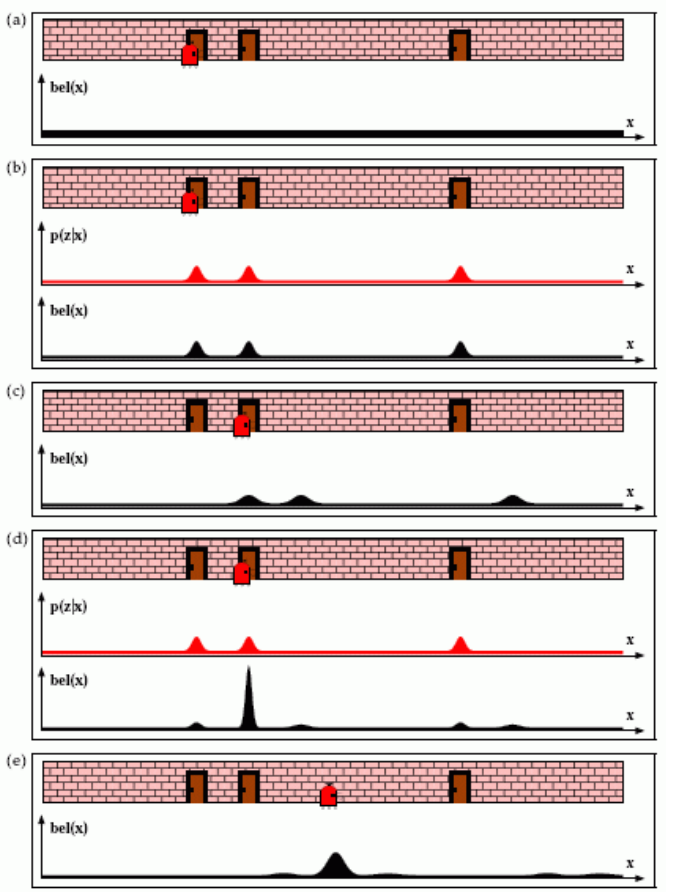
\includegraphics[scale=0.4]{Resources/PNG/MarkovAlgorithmus.PNG}
		\caption{Markov Algorithmus}
		\label{fig:Resources/PNG/MarkovAlgorithmus.PNG}
	\end{center}
\end{figure}
\newpage
\section{Monte Carlo Lokalisierung}
\subsection{Grundsätzliches Vorgehen}
\begin{itemize}
	\item Stichprobenbasierendes Approximationsverfahren
	\item Spezialform von Markov Lokalisierung
\end{itemize}
\begin{figure}[H]
	\begin{center}
		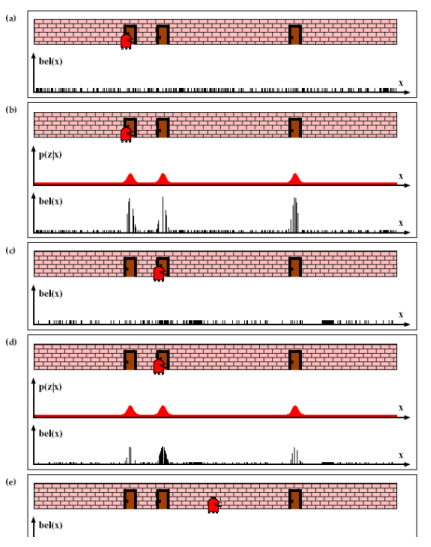
\includegraphics[scale=0.6]{Resources/PNG/MonteCarlo.PNG}
		\caption{Monte Carlo Lokalisierung}
		\label{fig:PNG/MonteCarlo.PNG}
	\end{center}
\end{figure}
\paragraph{Definition}
\begin{itemize}
	\item iterativer Bayesscher Filter, welcher als Schätzer für die zukünftige Wahrscheinlichkeitsverteilung der Roboterposition verwendet wird
	\item Unterscheidet sich im Gegensatz zu gridbasierten Lokalisierungsverfahren in der Betrachtung und in der Verarbeitung
	\subitem \textbf{Praxis}: viele der Gitterzellen besitzen Wahrscheinlichkeit von 0
	\subitem Miteinbeziehung dieser Gitterzellen in Berechnungen $\Rightarrow$ ineffizient
	\subitem diese können vernachlässigt werden
	\subitem fokusieren der Gitterzellen, die die wahrscheinlichsten Positionen widerspiegeln
\end{itemize}
\paragraph{Funktionsweise}
\begin{itemize}
	\item Positionsschätzung bei $(x_k)$ wird durch eine Menge von \textbf{Partikeln} dargestellt
	\item Es besteht keine Information über die Anfangsposition; Partikel sind \textbf{zufällig verteilt}
	\item Durch \textbf{Sensormessung $z$} werden die \textbf{Gewichte} (Strichhöhe) verändert
	\item \textbf{Resampling}: Aus der Partikelmenge werden zufällig aber entsprechend ihrem Gewicht Partikel gezogen $\Rightarrow$ integrierung des Steuerbefehls $(u_k)$ integriert.
	\item Es erfolgt eine erneute Gewichtung mit einem neuen Sensorwert
	\item Anschließend ein erneuetes Resamplung und Integrierung des Steuerbefehls
\end{itemize}
\paragraph{Vorteil}
\begin{itemize}
	\item zur Laufzeit kann die Größe der Stichprobenmenge variabel sein
	\item je unsicherer die Roboterposition ist, desto größer ist die Stichprobenmenge
\end{itemize}
\subsection{Partikelmengen}
\begin{itemize}
	\item Jeder Partikel stellt eine \textbf{Hypothese} für den \textbf{Zustand $x$} dar
	\item Generierung einer Partikelmenge X aus einer Wahrscheinlichkeitsichte p:
\end{itemize}
\begin{figure}[H]
	\begin{center}
		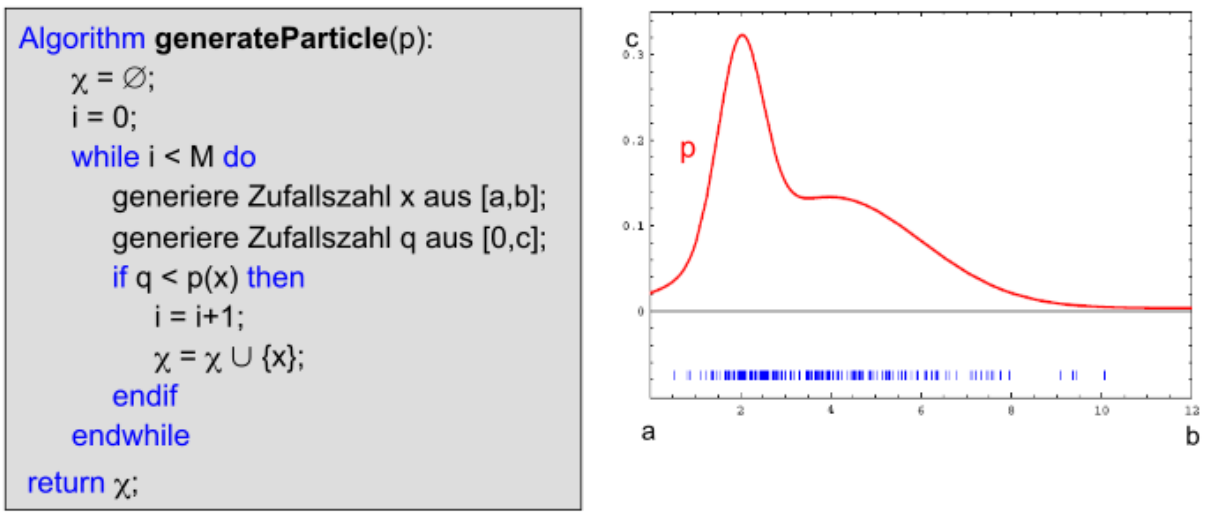
\includegraphics[scale=0.5]{Resources/PNG/PartikelMengen.PNG}
		\caption{Partikelmengen}
		\label{fig:PNG/PartikelMengen.PNG}
	\end{center}
\end{figure}
\section{Kalman-Filter}
\subsection{Definition}
\begin{itemize}
	\item Zustandsschätzer für dynamische Systeme
	\item Spezielle Version eines Bayes-Filters
	\item Dient zur Fusion von zwei unterschiedlichen, stochastisch unabhängigen Informationsquellen
\end{itemize}
\paragraph{Anwendung} fusion der Odometriedaten mit externen Messungen
\subsection{Vorgehen}
\begin{itemize}
	\item $Bel(x_t)$ wird durch seinen Erwartungswert $\mu$ sowie die Kovarianz $\sum_t$ approximiert.
	\item Zu jedem Zeitpunkt wird eine \textbf{Zustandsschätzung} geliefert, die aus einer Schätzung des aktuellen Zustandes und aus einer Vorhersage des Nachfolgezustandes nach Ausführung einer Aktion besteht.
	\item In die \textbf{Zustandsschätzungen} werden unabhängige Sensormessungen integriert
	\item In der \textbf{Vorhersagephase} benutzt der Kalman Filter die Zustandsschätzung vom vorhergehenden Zeitschritt um Zustandsschätzung für den aktuellen Zeitschritt zu erzeugen
	\item In der \textbf{Update} oder \textbf{Korrekturphase} werden die Messinformationen des aktuellen Zeitschritts verwendet, um die Vorhersage zu verbessern.
	\item Das Fehler Modell der Schätzung soll optimal aktualisiert werden auf Basis vorhandener Informationen
\end{itemize}
\subsection{Einschränkungen}
\begin{itemize}
	\item Fehlermodelle sind Gaußverteilungen
	\item Die Zustandsverteilung ist eine Gaußverteilung
\end{itemize}
\begin{figure}[H]
	\begin{center}
		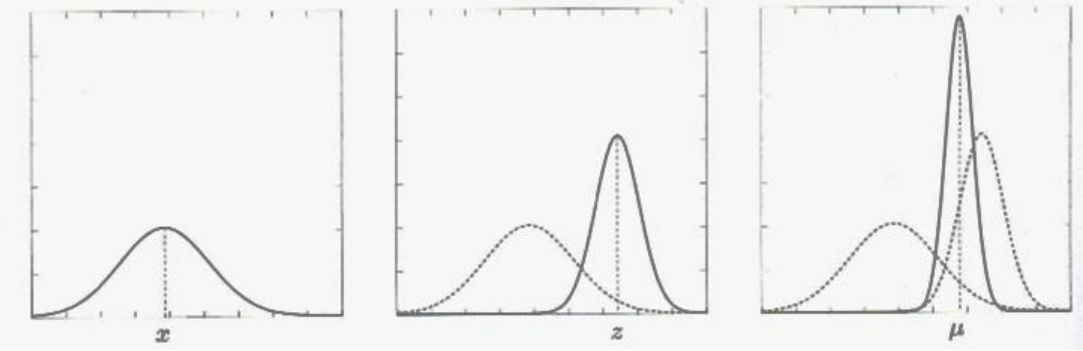
\includegraphics[scale=0.4]{Resources/PNG/KalmanFilter.PNG}
		\caption{Kalman Filter}
		\label{fig:PNG/KalmanFilter.PNG}
	\end{center}
\end{figure}
\begin{itemize}
	\item \textbf{Links}: Unsicherheit im aktuellen Zustand x
	\item \textbf{Mitte}: eine unabhängige Messung z liefert konkurrierende Informationen (\textit{Mittelwewrt und Varianz})
	\item \textbf{Rechts:} Fusion beider Daten liefert eine Mittelung, gewichtet mit der Sicherheit der Informationen, sowie reduzierte Varianz, d.h. eine größere Sicherheit in dem gefilterten Zustand
\end{itemize}
\section{Simultaneous Localization and Mapping}
\subsection{Landmarkenbasiertes SLAM Problem}
\paragraph{SLAM} Simultaneous Localization and Mapping
\begin{itemize}
	\item \textbf{Ausgangspunkt} Roboter exploriert eine unbekannte, statistische Umgebung
	\subitem Roboter kennt seine Pose (Position und Orientierung) nicht genau
	\subitem Es existiert keine Karte der Umgebung
	\item \textbf{Bekannt} sind Sensor- und Steuerdaten: $d = u_1, z_1, u_2, z_2 ... u_k, z_k$
	\item \textbf{Gesucht} Karte $m$ mit $M$ Landmarken: $m = l_1, x, l_1, y, ..., l_M,x,l_M,y$
	\item Weg des Roboters $x_1, x_2, ... x_k$
\end{itemize}
\paragraph{Probablisistische Algorithmen}
\begin{itemize}
	\item Ungenauigkeiten in den Messdaten werden durch Wahrscheinlichkeitsverteilungen modelliert
	\subitem bekannt sind die \textbf{Roboter Bewegungsbefehle} (die Kontrolldaten, die Steuerkommandos $u_t$)
	\subitem bekannt sind die \textbf{Beobachtungen} $z_t$ der nahe gelegnen \textbf{Landmarken} bestehend aus Entfernung und Winkel
	\subitem die Sensorik kann sowohl die Beobachtungsrichtung als auch die beobachtete Entfernung einer Landmarke zur Verfügung stellen
	\subitem gesucht ist eine Schätzung der Karte der Merkmale, der Landmarkenpositionen, sowie der Pfad des Roboters, d.h. seine aktuelle und frühere Posen
\end{itemize}
\subsection{Problemstellung}
\begin{itemize}
	\item Roboterpfad und Positionen der Landmarken in der Karte sind unbekannt
	\item Die Zuodnung von Messdaten zu Landmarken sind i.d. Regel unbekannt
	\item Roboter muss entscheiden, ob Messdaten einer bereits beobachteten Landmarke zugeordnet werden können oder einer noch nicht gesehenen Landmarke
	\item Problematik der Zuordnung wird durch Unsicherheit in der Roboterposition verstärkt
\end{itemize}
\begin{figure}[H]
	\begin{center}
		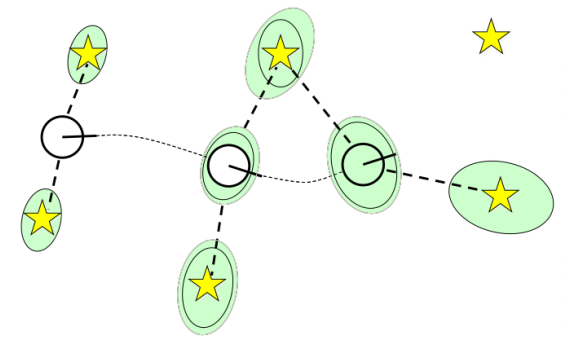
\includegraphics[scale=0.5]{Resources/PNG/ProbabilisitischeLandmarken.PNG}
		\caption{}
		\label{fig:PNG/ProbabilistischeLandmarken.PNG}
	\end{center}
\end{figure}
\subsection{Funktionsweise}
\begin{figure}[H]
	\begin{center}
		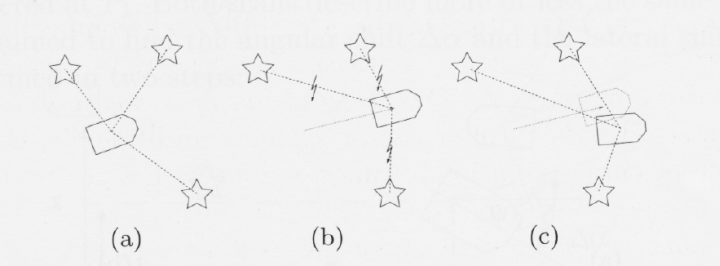
\includegraphics[scale=0.5]{Resources/PNG/FunktionsweiseSLAM.png}
		\caption{SLAM Darstellung}
		\label{fig:PNG/FunktionsweiseSLAM.png}
	\end{center}
\end{figure}
\begin{itemize}
	\item \textbf{(a)} Roboter misst Distanzen zu den Landmarken
	\item \textbf{(b)} Roboter schätzt seine neue Position anhand von Odometriedaten; Odometrie-basierte Roboterpose kann zur Schätzung der neuen Distanzen zu den in \textbf{(a)} verwendeten Landmarken herangezogen werden
	\item Nach Vergleich zwischen Roboter und Landmarken kann der Roboter seine Position \textbf{(c)} korrigieren
\end{itemize}
\subsection{Hinzunahme neuer Landmarken}
\begin{figure}[H]
	\begin{center}
		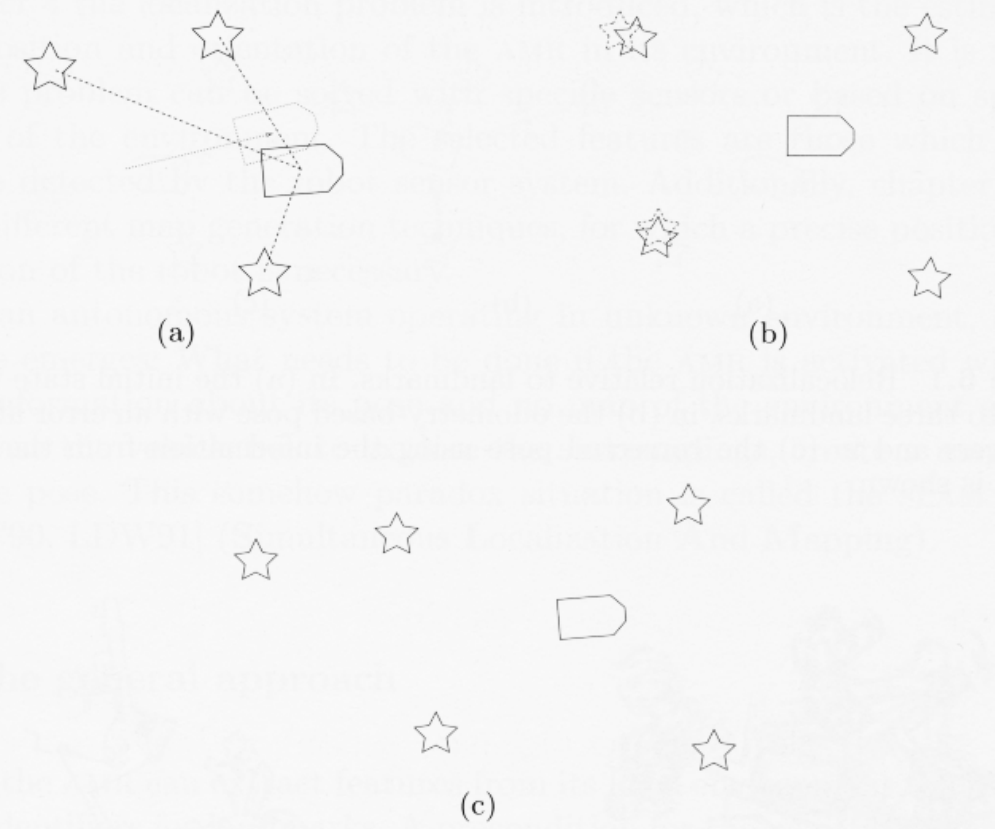
\includegraphics[scale=0.5]{Resources/PNG/LandmarkenErweitern.PNG}
		\caption{}
		\label{fig:PNG/LandmarkenErweitern.PNG}
	\end{center}
\end{figure}
\begin{itemize}
	\item (a) entspricht der Situation aus der vorhergehenden Folie.
	\item In (b) lokalisiert sich das Fahrzeug nach einer Bewegung erneut anhand zweier \enquote{alter} Landmarken und der letzten lokalen Karte
	\item Führt aufgrund der Fehler zu einer ungenauen, globalen Roboterposition
	\item Die Position der neuen Landmarken wird relativ zu der vermeintlich bekannten, korrekten Position der alten Landmarken bestimmt
	\item Positionsannahme ist inkorrekt
	\item Verschiebung der Position der \enquote{alten} Landmarken wird geschätzt und korrigiert sowie auf die Position der neuen Landmarken angewandt
\end{itemize}
\subsection{Aufbau eines SLAM-Graphen}
\begin{itemize}
	\item Sämtliche Messvorgänge sind fehlerbehaftet, auch die Positionsbestimmung der Landmarken
	\item Die Unsicherheit wird in der folgenden Abbildung als Fehlerellipse dargestellt.
	\item Roboter schätzt die Landmarken \textbf{A} und \textbf{B}
	\item nach Bewegung des Roboters nimmt die Genauigkeit der Lokalisierung ab
	\item Die Unsicherheit der Positionsschätzung der Landmarken \textbf{C} und \textbf{D} steigt
	\item Der Roboter erkennt eine bereits zuvor gesehene Landmarke
	\item Eine Verknüpfung mit der früheren Information über die Landmarke reduziert die Unsicherheit bei der Positionsbestimmung und damit auch die Unsicherheit über die zugehörigen früheren Roboterpositionen
\end{itemize}
\begin{minipage}[]{0.5\textwidth}
\begin{figure}[H]
	\begin{center}
		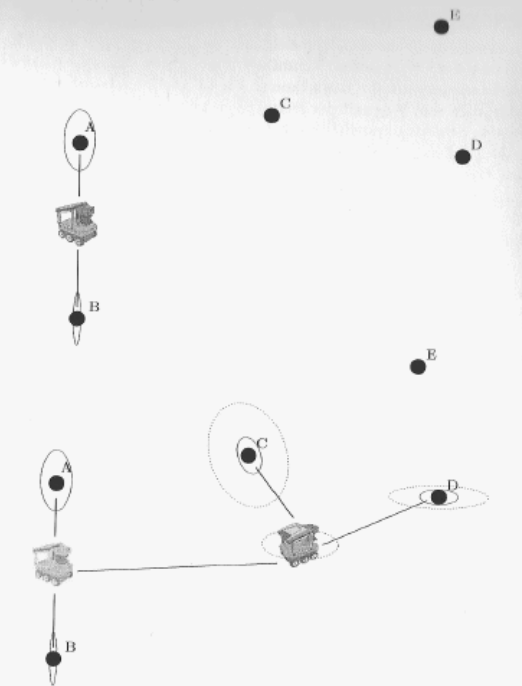
\includegraphics[scale=0.52]{Resources/PNG/LandmarkenBeispiel.PNG}
		\caption{}
		\label{fig:PNG/LandmarkenBeispiel.PNG}
	\end{center}
\end{figure}
\end{minipage}
\begin{minipage}[]{0.5\textwidth}
\begin{figure}[H]
	\begin{center}
		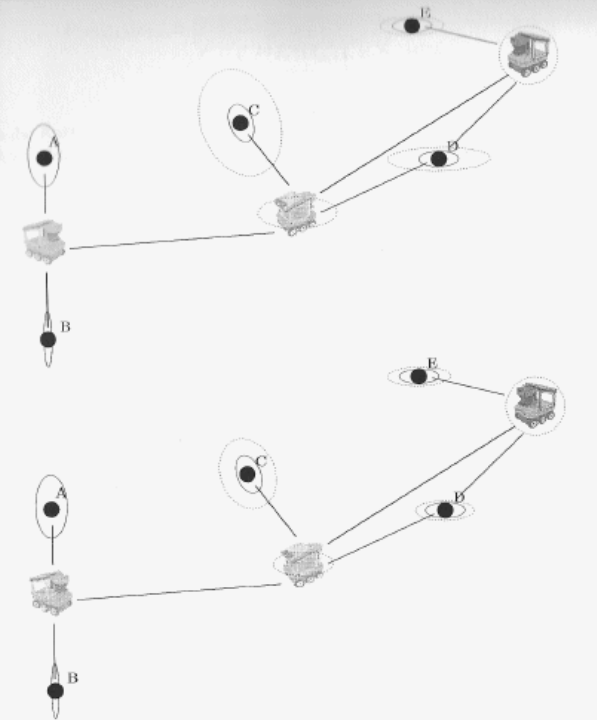
\includegraphics[scale=0.5]{Resources/PNG/LandmarkenBeispiel2.PNG}
		\caption{}
		\label{fig:PNG/LandmarkenBeispie2l.PNG}
	\end{center}
\end{figure}
\end{minipage}
\subsection{Varianten von SLAM}
\paragraph{Vollständiges SLAM}
\begin{itemize}
	\item Roboter schätzt eine Umgebungskarte $m$
	\item Roboter schätzt seine aktuelle Pose $x_t$ und \textbf{alle} zurückliegenden Posen $x_t-1$ bis $x_1$
	\item Grundlage sind die bisher wahrgenommenen Sensordaten $z_1:t$
	\item Sowie alle ausgeführten Aktionen $u_1:t-1$
	\item Es muss die Verteilung $P(m, x1:t | z_1:t, u1:t-1)$
\end{itemize}
\paragraph{Inkrementelles Slam}
\begin{itemize}
	\item Roboter schätzt nur die Karte $m$ sowie die aktuelle Position $x_t$
	\item Es muss die Verteilung $P(m, x_t | z1:t, u1:t-1)$ geschätzt werden
\end{itemize}
\subsection{Bayesian Netzwerk für landmarkenbasiertes SLAM}
\begin{itemize}
	\item Die einzelnen Landmarken sind unabhängig
	\item Gegeben sind die Roboterposen
\end{itemize}
\begin{figure}[H]
	\begin{center}
		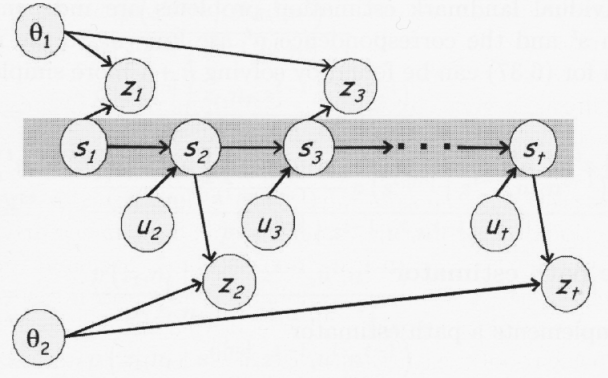
\includegraphics[scale=0.8]{Resources/PNG/BayesNetzwerk}
		\caption{Bayes Netzwerk}
		\label{fig:PNG/BayesNetzwerk}
	\end{center}
\end{figure}
Modell von Variablen und deren Abhängigkeiten als dynamisches Bayes-Netzwerk.
\begin{itemize}
	\item Kern des Modells bilden die
	\subitem Zeitreihe der Roboterzustände $s_1, s_2, ... s_t$
	\subitem die Positionen der Landmarken $\theta_k$
	\subitem die Kontrollvariablen $u_t$
	\subitem und die gemessenen, beobachteten Landmarken Positionen $z_t$
	\item Der Roboter bewegt sich von $s_1$ nach $s_t$ mit einer Folge Kontrolleingaben $u_2, ... u_t$
	%TODO Chapter 6 page 30
\end{itemize}





















